% Construct Validity Failure in Single-Cell Embedding Evaluation — poster v2
% tikzposter 3x3 block format, matching grokking_poster_v2.tex.
% All numbers from paper_d_v35.tex.
%
%   lualatex scib_poster_v2.tex

\documentclass[25pt, a0paper, portrait]{tikzposter}

\usepackage{amsmath,amssymb}
\usepackage{booktabs}
\usepackage{graphicx}
\usepackage{enumitem}
\usepackage{microtype}

\graphicspath{{../docs/figures/}}

% ── Color palette ───────────────────────────────────────
\definecolor{pass}{HTML}{27AE60}
\definecolor{warn}{HTML}{E67E22}
\definecolor{fail}{HTML}{E74C3C}
\definecolor{darktext}{HTML}{2C3E50}
\definecolor{blockbg}{HTML}{FFFFFF}

% ── Theme ───────────────────────────────────────────────
\usetheme{Default}

\definecolorstyle{SCIBColors}{
  \definecolor{colorOne}{HTML}{2C3E50}
  \definecolor{colorTwo}{HTML}{3498DB}
  \definecolor{colorThree}{HTML}{ECF0F1}
}{
  \colorlet{backgroundcolor}{colorThree}
  \colorlet{framecolor}{colorOne}
  \colorlet{titlefgcolor}{white}
  \colorlet{titlebgcolor}{colorOne}
  \colorlet{blocktitlebgcolor}{colorTwo}
  \colorlet{blocktitlefgcolor}{white}
  \colorlet{blockbodybgcolor}{blockbg}
  \colorlet{blockbodyfgcolor}{darktext}
  \colorlet{notefgcolor}{darktext}
  \colorlet{notebgcolor}{warn!15}
  \colorlet{notefrcolor}{warn}
}
\usecolorstyle{SCIBColors}

\defineblockstyle{SCIBBlock}{
  titlewidthscale=1.0, bodywidthscale=1.0, titleleft,
  titleoffsetx=0pt, titleoffsety=0pt,
  bodyoffsetx=0pt, bodyoffsety=0pt, bodyverticalshift=0pt,
  roundedcorners=12, linewidth=2pt, titleinnersep=10pt, bodyinnersep=15pt
}{
  \draw[rounded corners=\blockroundedcorners, color=blocktitlebgcolor,
        fill=blockbodybgcolor, line width=\blocklinewidth]
    (blockbody.south west) rectangle (blocktitle.north east);
  \ifBlockHasTitle
    \draw[rounded corners=\blockroundedcorners,
          fill=blocktitlebgcolor, color=blocktitlebgcolor,
          line width=\blocklinewidth]
      (blocktitle.south west) rectangle (blocktitle.north east);
  \fi
}
\useblockstyle{SCIBBlock}

\definetitlestyle{SCIBTitle}{
  width=\paperwidth, roundedcorners=0, linewidth=0pt, innersep=20pt,
  titletotopverticalspace=15mm, titletoblockverticalspace=25mm
}{
  \draw[fill=titlebgcolor, color=titlebgcolor]
    (\titleposleft, \titleposbottom)
    rectangle (\titleposright, \titlepostop);
}
\usetitlestyle{SCIBTitle}

\title{%
  \parbox{0.92\linewidth}{\centering\bfseries
    Construct Validity Failure in Single-Cell\\[3pt]
    Embedding Evaluation:\\[6pt]
    Null Saturation Bounds and Source Classifier Confidence}}
\author{Elliot Tower\quad\texttt{elliot@elliottower.ai}}
\institute{}

\begin{document}

\maketitle[width=\paperwidth]

% ════════════════════════════════════════════════════════
% ROW 1
% ════════════════════════════════════════════════════════
\begin{columns}
\column{0.33}

\block{The Problem}{
  Single-cell foundation model benchmarks consistently find that PCA on
  raw counts matches or exceeds large pretrained models across most
  evaluation axes. Whether this reflects a genuine limitation of current
  models or a \textbf{construct validity failure in the metrics} remains
  unresolved.

  \vspace{6mm}
  Embedding metrics serve two roles the field treats as one:
  \textbf{ranking} (which model is better?) and \textbf{certification}
  (does the model capture biological signal at all?). A metric can rank
  trained models correctly while scoring all of them below unstructured
  random noise.

  \vspace{6mm}
  We evaluated \textbf{twelve metrics} on \textbf{104 embedding
  conditions} across \textbf{25 tissues} in CELLxGENE Census, against
  cross-technology cell-type transfer F1 (10x Chromium 3$'$ v3
  $\to$ Smart-seq2).
}

\column{0.34}

\block{CKA Null Saturation}{
  Centered kernel alignment (CKA) on cell-type centroids retains
  ranking power (partial $\rho = 0.53$) yet exhibits \textbf{null
  saturation}: its analytic expectation under a Gaussian null is a
  closed-form function of $k$ cell types and embedding dimension $d$:

  \vspace{4mm}
  \begin{center}
  {\Large $\mathbb{E}[\mathrm{CKA}] \approx 1 - 1.06 \cdot \dfrac{k-1}{d+k}$}
  \end{center}

  \vspace{4mm}
  This formula matches simulation within 0.02\%. At foundation-model
  dimensionalities, the null exceeds every trained-model score:

  \vspace{4mm}
  \begin{center}
  \begin{tabular}{@{}rcc@{}}
    \toprule
    $d$ & \textbf{Above null} & \textbf{Total} \\
    \midrule
    50   & \textcolor{pass}{\textbf{218 (86\%)}} & 253 \\
    200  & \textcolor{warn}{\textbf{76 (17\%)}}  & 456 \\
    512  & \textcolor{fail}{\textbf{0 (0\%)}}    & 125 \\
    $\geq 768$ & \textcolor{fail}{\textbf{0 (0\%)}} & 4 \\
    \bottomrule
  \end{tabular}
  \end{center}

  \vspace{4mm}
  \textbf{Dimensionality is the causal variable.} scVI ($d = 50$, a
  foundation model) clears the null in 16/25 tissues. Bag-of-genes PCA
  at $d = 512$ fails in all 25.
}

\column{0.33}

\block{Dimensionality, Not Model Quality}{
  A PCA-reduction control confirms the mechanism. The same Geneformer
  embeddings, reduced from $d = 512$ to $d = 50$, shift from 0/22
  tissues clearing the null to 18/22.

  \vspace{5mm}
  \begin{center}
  \begin{tabular}{@{}lcc@{}}
    \toprule
    & $d = 50$ & $d = 512$ \\
    \midrule
    Foundation model & 16/25 (64\%) & 0/25 (0\%) \\
    PCA / random     & 86\%         & 0/25 (0\%) \\
    \bottomrule
  \end{tabular}
  \end{center}

  \vspace{5mm}
  To push the null below the observed CKA mean of 0.74 requires:

  \vspace{4mm}
  \begin{center}
  \begin{tabular}{@{}rrl@{}}
    \toprule
    $d$ & $k$ needed & Feasibility \\
    \midrule
    50   & $> 18$  & Routine \\
    200  & $> 66$  & Rare \\
    512  & $> 168$ & Beyond any dataset \\
    1280 & $> 417$ & Infeasible \\
    \bottomrule
  \end{tabular}
  \end{center}
}

\end{columns}

% ════════════════════════════════════════════════════════
% ROW 2
% ════════════════════════════════════════════════════════
\begin{columns}
\column{0.33}

\block{Metric Prediction of Transfer}{
  Nine of twelve metrics significantly predict cross-technology transfer
  (partial $\rho$, controlling for dimensionality):

  \vspace{4mm}
  {\small
  \begin{tabular}{@{}lcc@{}}
    \toprule
    \textbf{Metric} & $\rho$ & $p$ \\
    \midrule
    Procrustes similarity & $+0.65$ & $< 10^{-4}$ \\
    Silhouette (target)   & $+0.65$ & $< 10^{-4}$ \\
    Graph connectivity    & $+0.58$ & $< 10^{-4}$ \\
    NMI (Leiden)          & $+0.55$ & $< 10^{-4}$ \\
    Cell-type CKA         & $+0.53$ & $< 10^{-4}$ \\
    kNN purity            & $+0.52$ & $< 10^{-4}$ \\
    ARI (Leiden)          & $+0.37$ & $< 10^{-4}$ \\
    Direction stability   & $+0.02$ & $0.83$ \\
    \bottomrule
  \end{tabular}
  }

  \vspace{4mm}
  Predictive validity does not imply discriminative validity. A metric
  can rank correctly while every score sits below random noise.
}

\column{0.34}

\block{Source Classifier Confidence (SCC)}{
  SCC trains a cell-type classifier on source embeddings, applies it to
  target cells, and reports the mean maximum predicted probability. It
  directly measures whether learned decision boundaries transfer.

  \vspace{5mm}
  {\small
  \begin{tabular}{@{}lccc@{}}
    \toprule
    \textbf{Classifier} & $\rho$ & 95\% CI & Pairwise \\
    \midrule
    SCC (LR)  & $\mathbf{+0.77}$ & $[+.64,\;+.85]$ & 82.6\% \\
    SCC (kNN) & $+0.51$          & $[+.31,\;+.66]$ & 78.3\% \\
    SCC (RF)  & $+0.59$          & $[+.38,\;+.74]$ & 79.7\% \\
    SCC (SVM) & $+0.52$          & $[+.30,\;+.69]$ & 72.5\% \\
    \bottomrule
  \end{tabular}
  }

  \vspace{5mm}
  All four classifier families pass BH correction ($p < 0.001$). The
  cross-classifier consistency rules out a shared-machinery confound:
  SCC measures an \textbf{embedding-space property}, not a classifier
  artifact.
}

\column{0.33}

\block{Convergent Validity}{
  SCC predicts marker gene recovery---a non-classification ground truth
  scored in gene space via Leiden clustering:

  \vspace{5mm}
  \begin{center}
  Spearman $\rho = 0.32$

  \vspace{2mm}
  Block-bootstrap 95\% CI: $[0.15,\; 0.44]$
  \end{center}

  \vspace{5mm}
  This provides convergent validity from a structurally distinct
  evaluation pathway: classifier confidence in embedding space predicts
  marker gene recovery in gene space.

  \vspace{5mm}
  Relational consistency scores (RCS), which operate on $k \times k$
  cell-type relationship matrices, are dimensionality-stable yet predict
  transfer only marginally ($\rho \leq 0.32$). Geometric similarity
  between cell-type relationship matrices does not reflect cluster
  separability.
}

\end{columns}

% ════════════════════════════════════════════════════════
% ROW 3
% ════════════════════════════════════════════════════════
\begin{columns}
\column{0.33}

\block{Pairwise Inversion Rates}{
  \begin{center}
  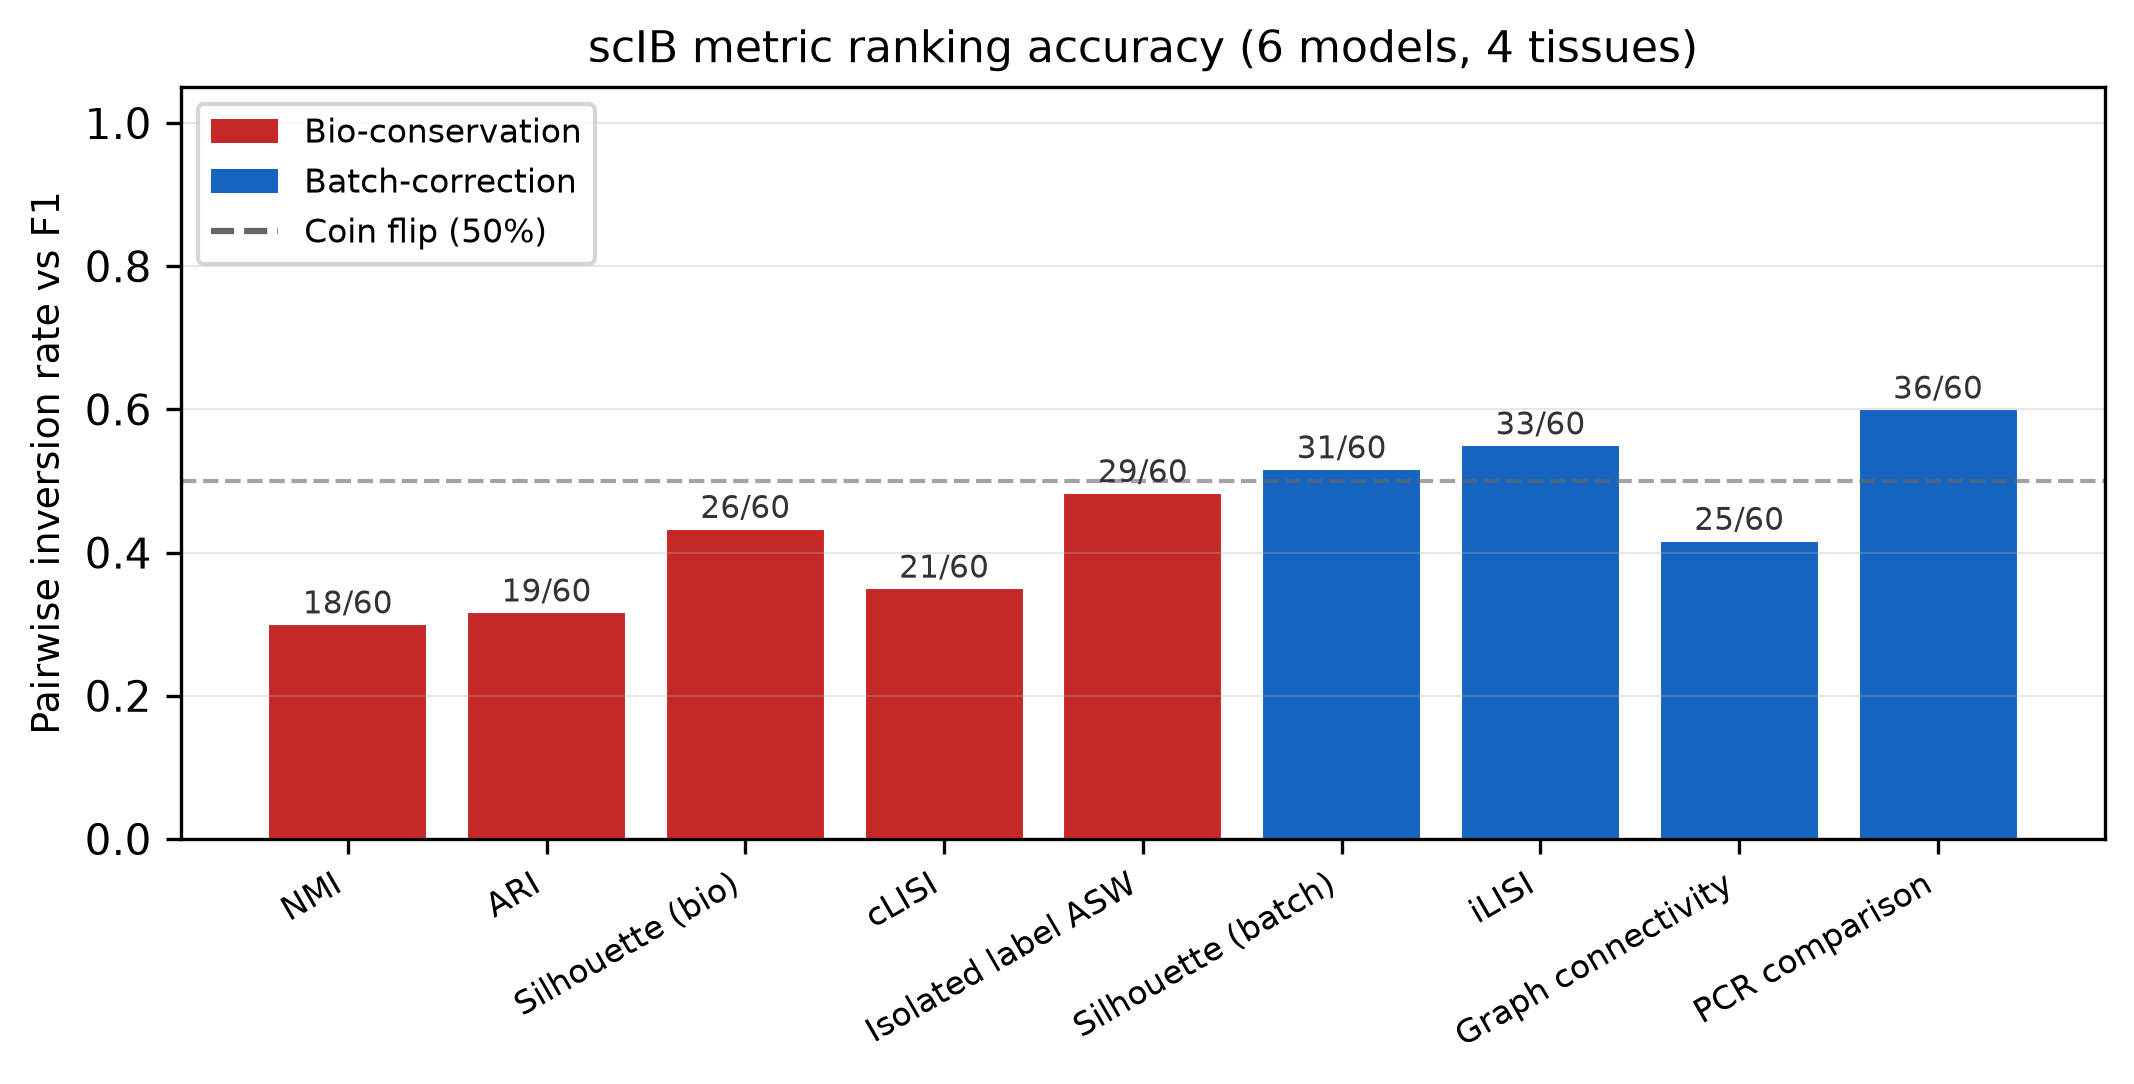
\includegraphics[width=0.95\linewidth]{inversion_rates.pdf}
  \end{center}

  \vspace{3mm}
  {\small Bio-conservation metrics show 30--48\% pairwise inversion
  rates on cross-assay transfer, at or near the 50\% coin-flip line.
  An inversion: a metric ranks model A above B, but transfer F1
  ranks them in the opposite order.}
}

\column{0.34}

\block{Clustering Jitter}{
  Leiden-dependent scIB metrics (NMI, ARI) show apparent
  non-monotonicity across embedding quality. Multi-seed noise
  calibration (10 seeds, 22 tissues) reveals this is
  \textbf{clustering jitter}:

  \vspace{5mm}
  ARI non-monotonicity drops from 70\% to 6.7\% after permutation
  calibration---a $10.5\times$ inflation.

  \vspace{5mm}
  Cross-tissue replication localizes the failure: scIB metrics achieve
  22\% pairwise inversions on cross-tissue transfer ($\rho = +0.63$,
  $p = 0.0014$), compared with 30--48\% in cross-assay. Protocol
  artifacts confound the cross-assay setting.

  \vspace{5mm}
  Three independent cell-sampling seeds produce inversion rates of
  22.1\%, 22.2\%, and 17.8\% (cross-tissue), confirming seed stability.
}

\column{0.33}

\block{Takeaway}{
  \textbf{Relational embedding metrics quantify geometric fidelity,
  which does not capture the cluster separability that determines
  downstream classification performance.}

  \vspace{6mm}
  \begin{itemize}[leftmargin=*, itemsep=4mm]
    \item CKA null saturation is a closed-form function of $k$ and $d$;
      at $d \geq 512$, zero conditions clear the null
    \item Dimensionality, not model quality, drives the boundary
    \item SCC achieves $\rho = 0.77$ with transfer F1, robust across
      four classifier families
    \item SCC predicts marker gene recovery ($\rho = 0.32$), a
      non-classification ground truth
    \item Published benchmark rankings derived from relational metrics
      alone warrant re-evaluation
  \end{itemize}

  \vspace{8mm}
  \begin{center}
  \texttt{elliot@elliottower.ai}

  \vspace{3mm}
  {\small 8 models $\cdot$ 25 tissues $\cdot$ 104 conditions $\cdot$
  CELLxGENE Census}
  \end{center}
}

\end{columns}

\end{document}
